\documentclass[12pt]{exam}
\usepackage[utf8]{inputenc}
\usepackage{amsmath,amssymb}
\usepackage{graphicx}

\begin{document}
	
	\begin{center}
			\LARGE{\textbf{Web Template}}
	\end{center}
	The section covers the basic information regarding template design and specifications. The templates are temporary due to the stage of the project, a new and improved template will be design for the final stage. 
\section{Wireframe}
All pages use a standardize background template. The background template contains a Texas Tech University white banner on top and Texas Tech Dark Red for the background color.
\subsection{Sign-In}
The sign-in template contains the standard background template and sign-in box.
\begin{center}
\emph{\\}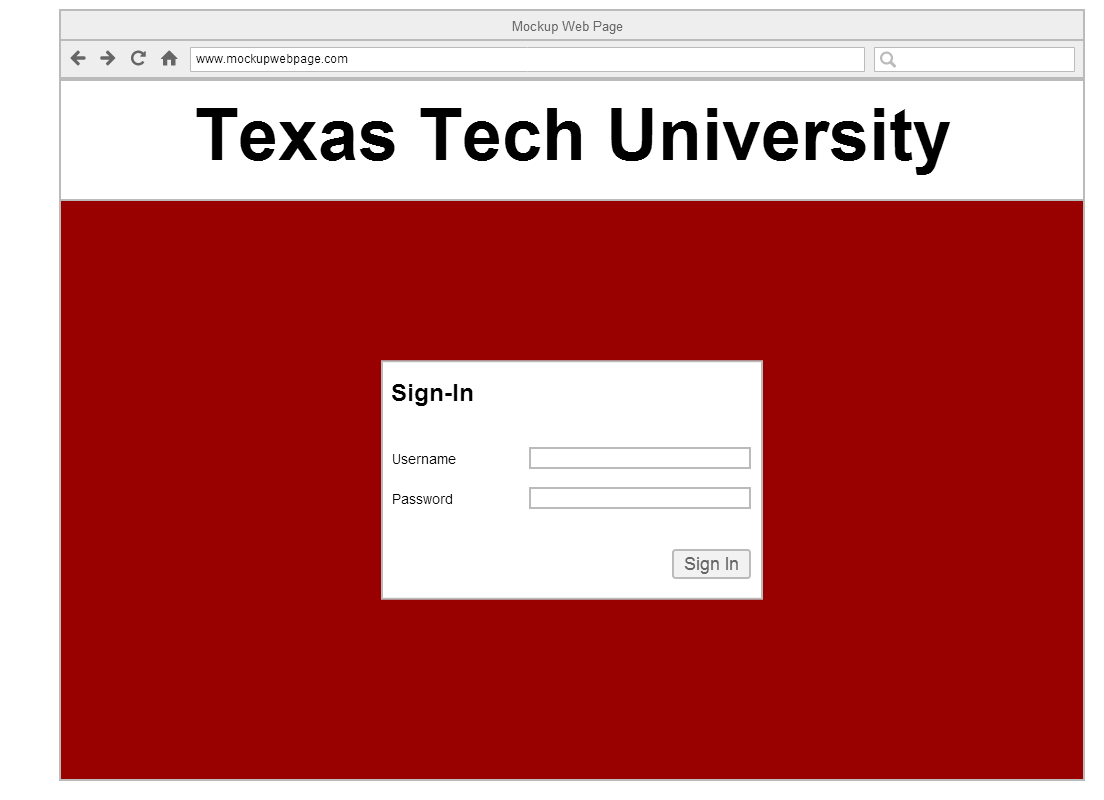
\includegraphics[scale=0.20]{signin.PNG}\\
\end{center}
	
\subsection{Display}
The display template contains the standard background template and output chart.
\begin{center}
\emph{\\}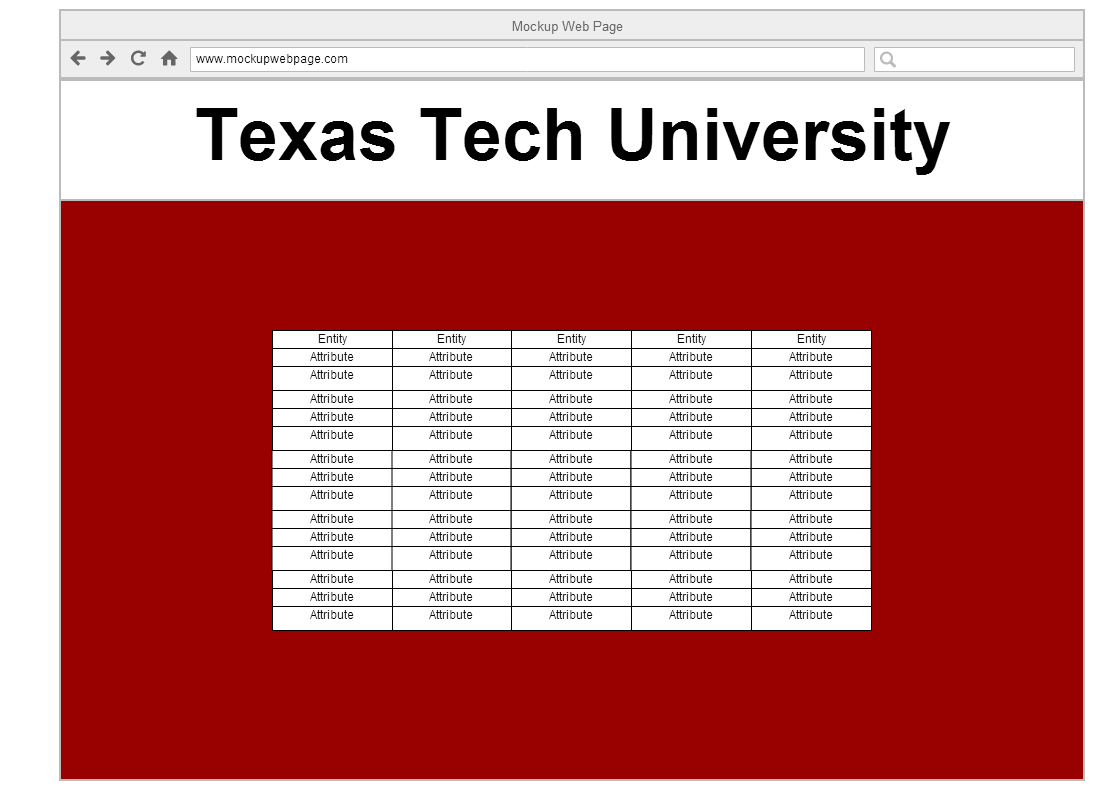
\includegraphics[scale=0.20]{display.PNG}\\
\end{center}

\section{Typography}
The typefaces style has been written to automatically format attractive, readable headers and paragraphs with the following substitutions:\\

\noindent\textbf{High-level headers and some major introductory paragraphs}\\
Arial\\

\noindent\textbf{General content and lower-level headers}\\
Arial

\section{Color}
The page template colors are Texas Tech Dark Red and Texas Tech Black official colors. This is the primary palette used to represent Texas Tech University.	

\begin{center}
\emph{\\}\includegraphics[scale=0.30]{capture.PNG}\\
\end{center}

\end{document}
